
\chapter{Background}\label{background}

%%

\section{Compilers and Interpreters}\label{compilers}
The execution of a program's source code is normally done using a compiler or an interpreter\cite{compilers-interpreters}. A compiler takes the source code and transforms the source code into a different representation - normally a series of bytes corresponding to machine instructions - to be executed on a machine or special program. An interpreter parses the program source code and executes the code directly according to the language specification.

\section{The C Programming Language}

C was created in 1972 at Bell Labs\cite{ritchie1993development} to write programs for Unix. The language grew massively after being used to re-write the Unix kernel and thus becoming the de-facto language of Unix. The language was based upon B\footnote{And led to an inspiring choice of name for the language.} and was designed as a low-level, system programming language. The C standard was brought into place by an international committee\cite{iso_standard} and defines the syntax and semantics of the language that compilers of the language should adhere to.

Here is a short C program that prints the Fibonacci sequence to show basic C syntax.

\begin{lstlisting}[language=C, caption=Example C program]
#include <stdio.h>
int main(int argc, char *argv[]) {
    int i, n = argc, a = 0, b = 1, c;
    for (i = 0; i < n; ++i) {
        printf("%d, ", a);
        c = a + b;
        a = b;
        b = c;
    }
    return 0;
}
\end{lstlisting}

\subsection{Characteristics of C}
One of the more prominent features of C is the languages extensive use of pointers\cite{tutorials-point}; values which point to objects in the programs memory. These objects can range from a single integer to arrays of pointers each pointing to complex \texttt{structs}. Structs are C's simpler versions of classes that are often seen in object oriented languages. They allow the program to define a data type that groups together one or more\footnote{Most compilers will allow compilation of empty structs and generate a warning about the empty struct.} types.

\begin{multicols}{2}
    C makes use of both the stack and the heap to store objects. Local variables are usually defined on the stack whilst global variables and dynamically allocated objects are placed on the heap. A programs memory typically has the following segments laid out.

    \begin{itemize}
    \item Text segment - where executable code is stored
    \item Initialized data segment
    \item Uninitialized data segment
    \item Stack
    \item Heap
\end{itemize}

\begin{center}
    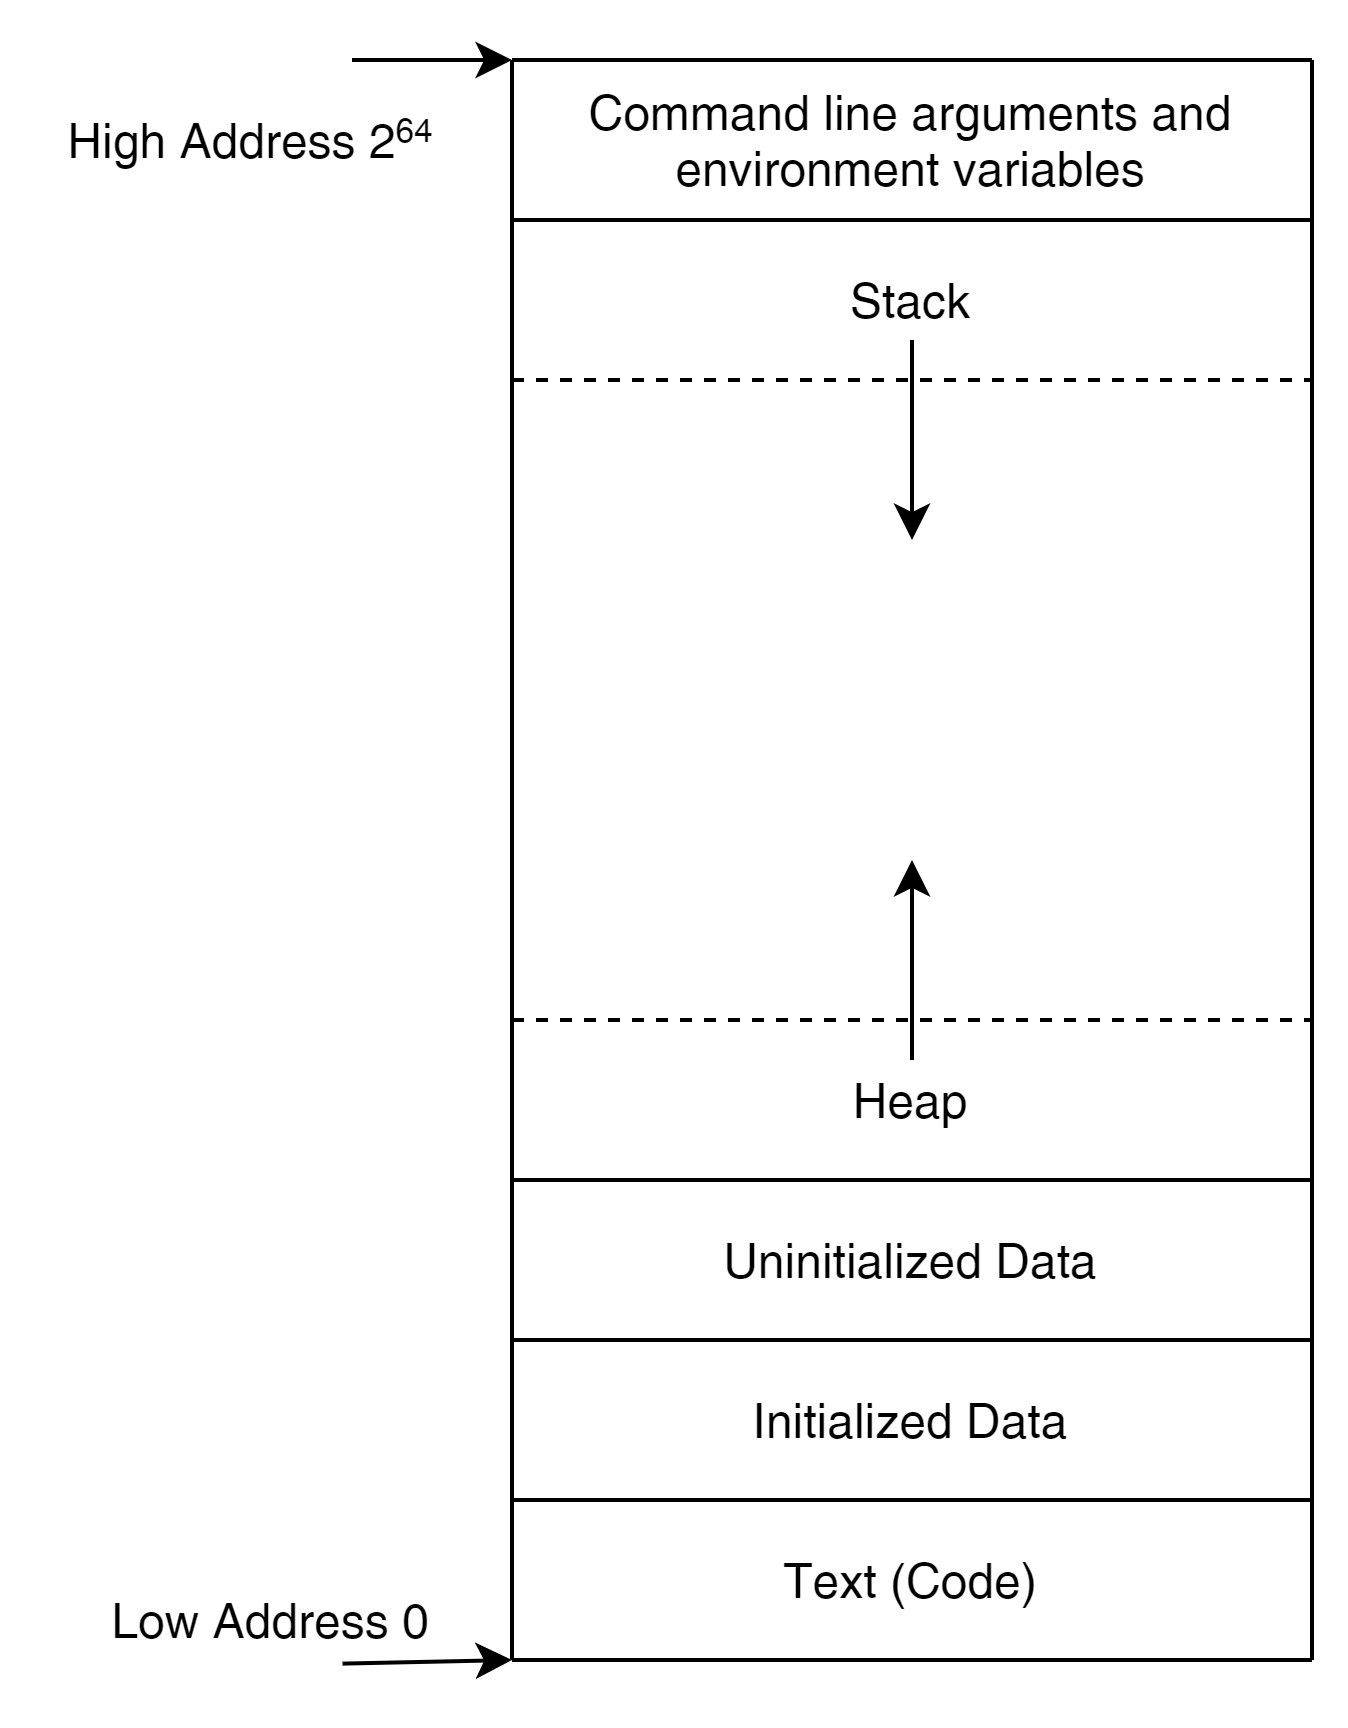
\includegraphics[height=0.4\textheight]{stack.png}
\end{center}
\end{multicols}

Accessing array and struct elements in C is done by calculating the offsets from the pointer to the base of the object to the element. For example, integers are \texttt{4} bytes, so accessing the \nth{10} element of an integer array would be done by calculating $\texttt{addr} + 10*4$.


\subsection{Problems with C Code}

Code written in C has a history of being \textit{very} bug prone\cite{common-bugs}. Due to the language's popularity and speed it is often used in security-critical applications. Many vulnerabilities that appear in C code are to do with incorrect memory management. The most common examples are dereferencing unknown memory locations, buffer overflows, accessing previously freed memory, reading uninitialized memory and double freeing a memory location.

The first example shows and example of an uninitialized pointer.

\begin{lstlisting}[language=C, caption=Dereference unknown memory location]
int main(){
    int *x;
    x[0] = 1;
    return 0;
}
\end{lstlisting}

\texttt{x} is uninitialized and points to a random place in memory, thus dereferencing \texttt{x} will result in undefined behaviour and most likely a segmentation fault.

The next example shows a classic buffer overflow, \texttt{strcpy} copies the memory at the location of the second argument to the location of the first argument until a null byte (\texttt{\char`\\x00}) is found in the input string.

\begin{lstlisting}[language=C, caption=Buffer overflow]
#include <string.h>
#include <stdlib.h>
int main(){
    char buf[4];
    char str[] = "Hello World!AAAAAAAAAAAAAAAAAAAAAAAAAAAAA";
    strcpy(buf, str);
    return 0;
}
\end{lstlisting}

Strings in C have a null byte at the end of string, which is called a \textit{null-terrminated string}. Thus the \texttt{strcpy} will attempt to copy the entirety of \texttt{str} into \texttt{buf}, overflowing \texttt{buf} and overwriting the memory addresses above \texttt{buf}. Because these variables are allocated onto the stack the overwritten memory could contain the current functions return address and allow control-flow hijacking by a malicious actor. This can lead to remote code execution on the target system.

The C11 standard defines five memory management functions\cite{iso_standard}, \texttt{aligned\_alloc}, \texttt{calloc}, \texttt{malloc}, \texttt{realloc} and \texttt{free}. The standard places a number of guarantees on the memory management.
\begin{itemize}
    \item Returned pointers are suitably aligned so that the space can be used for type casting.
    \item The lifetime of an allocated object is defined between the objects allocation and deallocation. The state of the object outside of these bounds is undefined.
    \item Each allocation will yield a pointer to an object disjoint from any other memory object.
    \item The returned pointer will point to the lowest address of the allocated memory.
    \item If the requested memory size is zero, then the behaviour is implementation specific and either a null pointer or the implementation will behave as if the size is non-zero with the catch that the resultant pointer is not used for memory access to an object.
\end{itemize}

Applying the guarantees to the example below shows how memory that has been freed or de-allocated can have unintended effects when accessed. 

\begin{lstlisting}[language=C, caption=Access previously freed memory, label={code:access_freed}]
#include <stdlib.h>
#include <stdio.h>
int main(){
    int *x;
    x = malloc(sizeof(int)*32);
    x[0] = 1;
    free(x);
    int *y = malloc(32*sizeof(int));
    y[0] = 2;
    printf("%d", x[0]);
    return 0;
}
\end{lstlisting}

There are no guarantees on the state of the region associated with \texttt{x} after the \texttt{free} call and thus any succeeding accesses to \texttt{x} are undefined. Then, when the object \texttt{y} is allocated, the object can be allocated to a non-disjoint region from the region for \texttt{x}. Thus, in some\footnote{depending on libc and operating system implementation} environments \texttt{y[0]=2} will override the value of \texttt{x[0]} and "2" will be printed.

The last class of undefined behaviour that shall be covered in this section is the double free. Double free's root cause is the same as Listing \ref{code:access_freed} with a different manifestation.

\begin{lstlisting}[language=C, caption=Double free, label={code:double-free}]
#include <stdlib.h>
#include <stdio.h>
int main(){
    int *x;
    x = malloc(4*sizeof(int));
    x[0] = 1;
    free(x);
    int *y = malloc(10*sizeof(int));
    y[0] = 2;
    free(x);
    return 0;
}
\end{lstlisting}

From the previous example it is possible for \texttt{x} and \texttt{y} to point to the same region of memory after the allocation of \texttt{y}, thus freeing \texttt{x} again will actually free a subregion \texttt{y} the size of the of \texttt{x}. In this case a region of size 4 at will be de-allocated.

\subsection{Detecting Undefined Behaviour in C Using Static Tools}
For performance and safety critical code, static analysis of code is the primary means of verifying the correctness and identifying undefined behaviour in a programs execution\cite{jourdan2015formally}.

The analysis for a given program is performed on the source code exclusively, and does not involve executing any part of the program. Various methods such as symbolic execution, model checking and data-flow analysis have achieved good accuracy at detecting undefined behaviour but due to the undecidability of the Halting problem there is no correct mechanical method for determining if a general program has undefined behaviour\footnote{There is a simple reduction from deciding whether a program will execute undefined behaviour to the Halting problem}.  

\subsection{Detecting Undefined Behaviour in C Using Dynamic Tools}
Dynamic analysis varies from static analysis by running the program on a real or virtual processor. Most dynamic analysis tools monitor the state of the program and track variable values and memory accesses for invalid operations. Depending on the type of analysis required different tools have different priorities. A security tool will "fuzz" the program and supply a large number of inputs to hunt down invalid operations while a performance tool will be more concerned with cpu time spent on functions and building a time based control-flow of the program. 

An example tool is Valgrind~\cite{seward2005using} which is an extensible framework for dynamic analysis and has inbuilt tools for memory debugging and detecting invalid malloc and free calls.

\section{Coq and Formal Verification}

\begin{quotation}
    \textit{`Coq is a formal proof management system. It provides a formal language to write mathematical definitions, executable algorithms and theorems together with an environment for semi-interactive development of machine-checked proofs.'}~\cite{coq_website}.
\end{quotation}

Whilst this project does not involve any writing of the Coq language there has been a large amount of \textit{reading} of Coq in this project due to CompCert being largely written in Coq. Coq has a large range of uses. For example, formally verifying that a compiler will produce a program that conforms to the specified execution even through optimizations (otherwise known as operational semantics) and formalizing and proving mathematical theorems. I will present an example from "A short introduction to Coq"\cite{introduction-to-coq} to show how a proposition for even and odd numbers would be written.

\begin{lstlisting}[language=Coq, caption=Coq definition of even and odd numbers]
Inductive even : N -> Prop :=
  | even_0 : even 0
  | even_S n : odd n -> even (n + 1)
  with odd : N -> Prop :=
  | odd_S n : even n -> odd (n + 1).
\end{lstlisting}

This is an example of a \textit{proposition} in Coq. Propositions are statements that can either be true or false. The other category of objects found in Coq are \textit{types}. Types are typically used for executable algorithms and mathematical definitions, whereas propositions are commonly used to define relations between states.

The Coq system has a functional programming language that supports these types and can be used to write programs. Furthermore, the programming language has an extraction feature\cite{coq-extraction} which allows Coq code to be extracted to certified and efficient functional programs. Coq currently has three output languages; OCaml\cite{leroy2014ocaml}, Haskell\cite{jones2003haskell} and Scheme\cite{dybvig2009scheme}. The CompCert compiler / interpreter that the project is using is extracted to OCaml and as such is the only extraction needed for the project. Coq can extract a series of Coq (\texttt{.v}) files to either a singular monolithic OCaml (\texttt{.ml}) file or separately extract each \texttt{.v} file to a corresponding \texttt{.ml} file\cite{coq_extraction}. The latter becomes much more appealing as the scale of the program grows and wrapper code can abstract out larger parts of the extracted program. The wrapper code is written in OCaml and can load any of the extracted OCaml modules. Once all OCaml code has been extracted / written all of the OCaml files can be compiled and linked to form an executable.

A number of the C semantics that I will be talking about further on in the project are propositions and defined as relations between states and can not be extracted out to OCaml.

\section{CompCert}\label{compcert}

\begin{quotation}
    \textit{
    `The CompCert project investigates the formal verification of realistic compilers usable for critical embedded software. Such verified compilers come with a mathematical, machine-checked proof that the generated executable code behaves exactly as prescribed by the semantics of the source program.'}~\cite{noauthor_compcert_nodate}
\end{quotation}
    CompCert's way of modelling memory is of key interest. The current version of CompCert models memory as a collection of \texttt{blocks}, each block modelling an area of memory in the program. The start and end points of each block are defined by  \texttt{low\_bound} and \texttt{high\_bound}, with pointers being represented by  $(b,i)$ pairs (the block identifier $b$ and an offset $i$). Pointer arithmetic is bounded by \texttt{low\_bound} and \texttt{high\_bound}. Attempting to access memory outwith the bound for a given block is an instance of \textit{undefined behaviour}. There are many other ways to encounter undefined behaviour (as defined in the C11 standard)\cite{iso_standard}.
    
    % The collection of blocks are contained in the \texttt{mem} type (with constant \texttt{empty : mem} denoting the empty state) and there are 7 operations that can be performed upon the memory:
    
    % \texttt{alloc, free, load, store, loadbytes, storebytes, drop\_perm}
    
    % the \texttt{drop\_perms} operation is special as it lowers the permission over a range of bytes. Details on permissions can be found in the relevant paper\cite{leroy2012compcert}.
    \begin{center}
        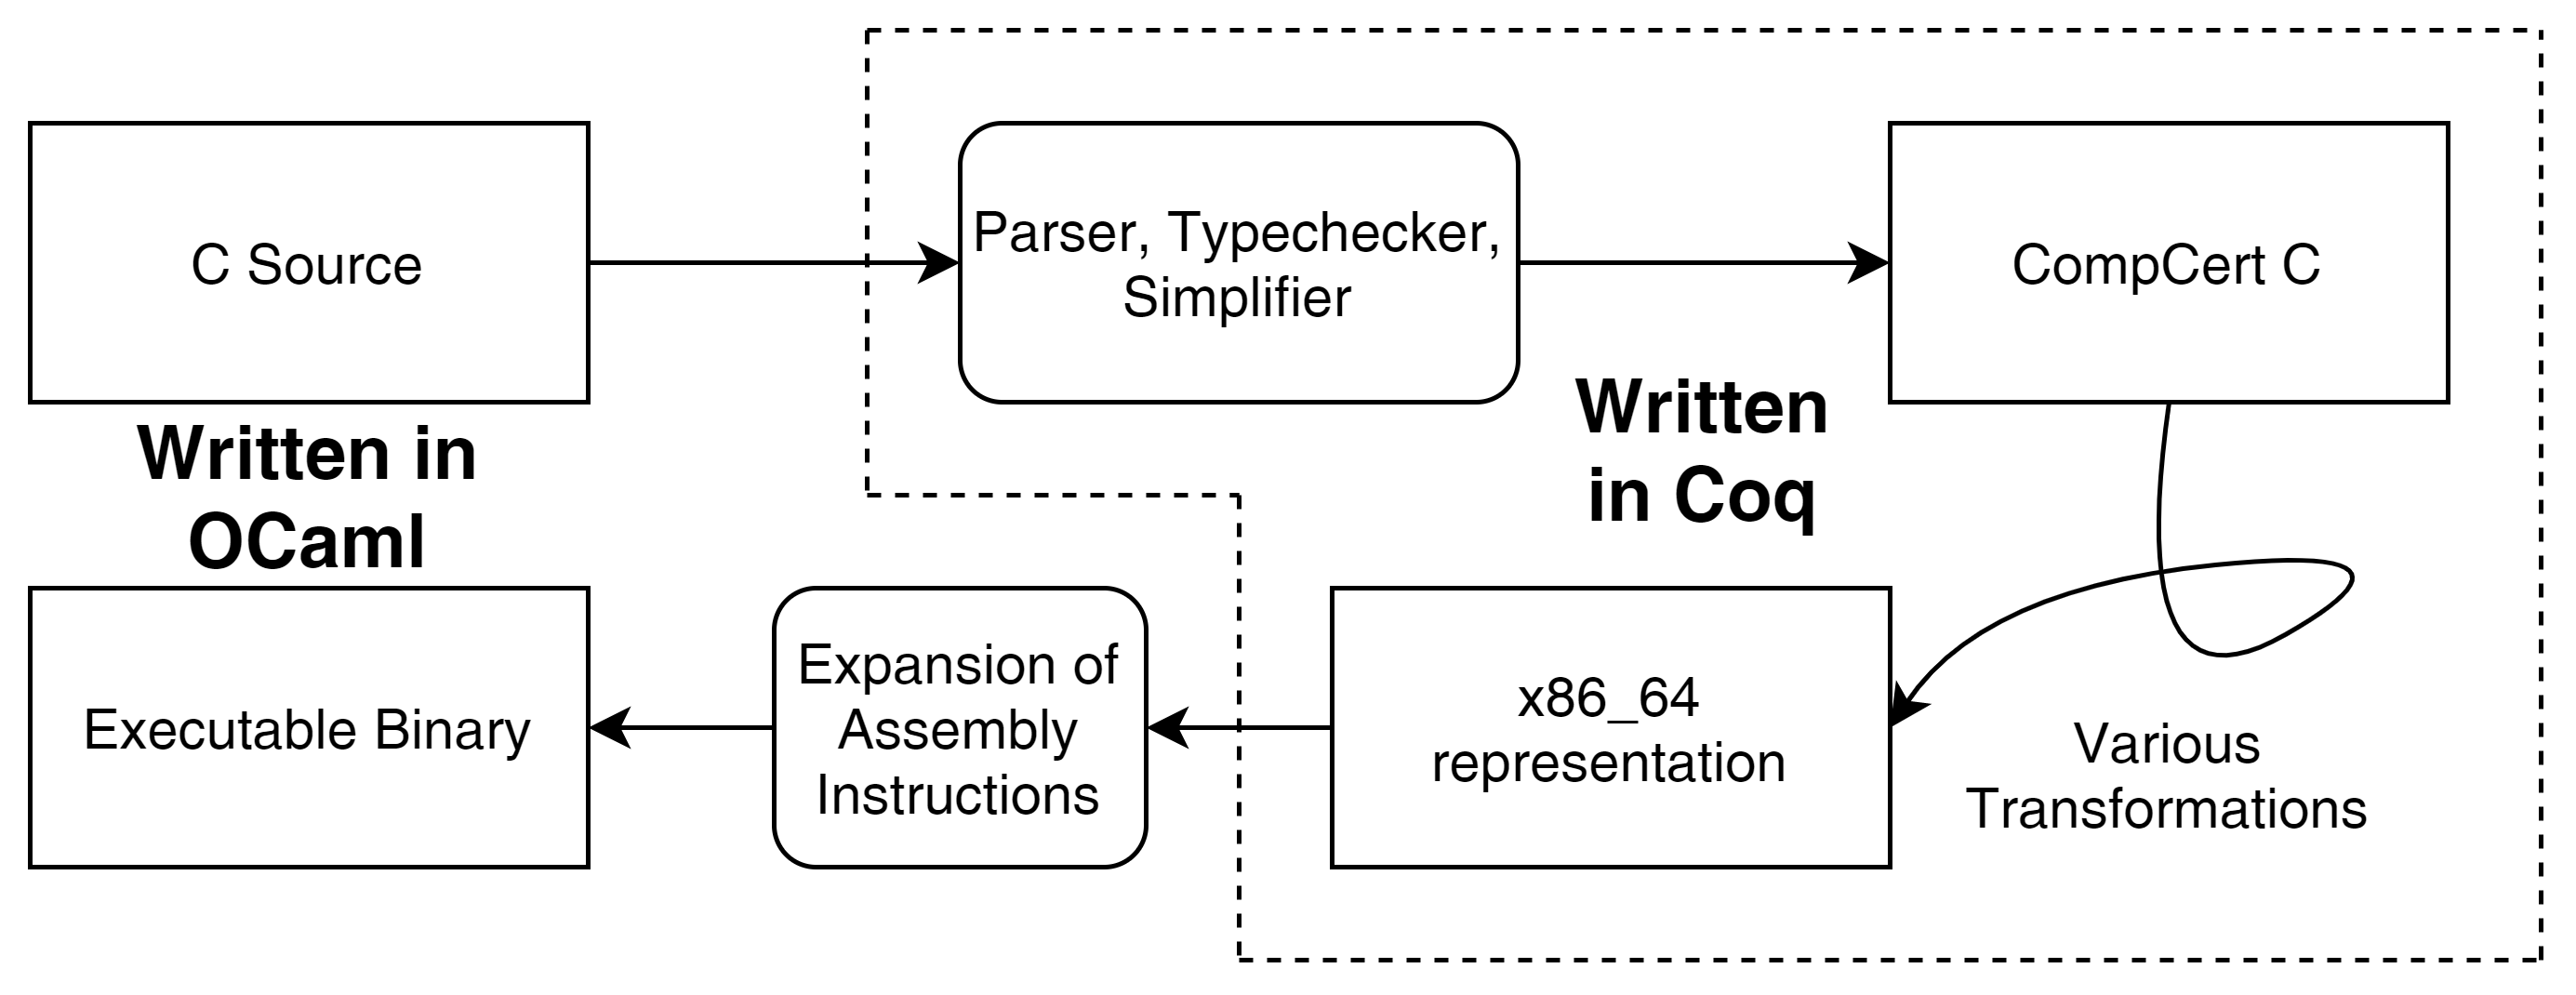
\includegraphics[width=0.8\textwidth]{ccomp-graph.png}
    \end{center}
    
    Instructions in CompCert are target platform specific and are defined in the respected target architecture's Coq Asm definition. For this project the x86\_64 architecture was chosen as the development machines are running on x86\_64 architecture and this will speed development time, there are also many tools available for x86\_64 due to it's abundance
    . The instructions build upon the abstract register types so that they can be reasoned about formally at compile time. Not all instructions are defined for the target architecture, and some operations are reduced into a simplified form (such as frame allocation). These reduced instructions are expanded when the program is emitted (interestingly, the expansion is not defined formally).
    
    Instruction execution is defined as operations over the register set, world state and memory state and is used in the compiler for verifying correctness over the compilation step.
    
    % The CompCert interpreter is given the program as . We can visualize CLight as a symbolization of the C source, such that every line of text, i.e. \texttt{int x = 1;} is represented more like $x : \texttt{int} \leftarrow 1$, a more abstract form. The interpreter then executes each line of code in a virtual model according to the C specification.
    
    % The CLight representation is where the compiler can perform static analysis, prove the correctness of a program and do model checking. These analysis's can be used by the interpreter as they are performed on the CLight representation without modifying it. 
    
    % This differs from the compilation step which introduces optimizations and produces a set of x86\_64 instructions that are emitted into a file.
    
% \section{Static Analysis of Source Code}\label{static-analysis-of-source-code}


% % \section{Dynamic Analysis}\label{dynamic-analysis}

\section{Disassembling}\label{disassembling}
In the context of this project disassembling refers to transforming machine code (i.e. bytes) into human-readable assembly. There are many existing tools with varying features sets that perform this task\cite{brumley2011bap, objdump, gdb} to varying degrees of complexity. Simple disassemblers are concerned with recreating the instructions while more complex programs attempt to reconstruct the control flow graph of the program and attempt to infer the semantics of the program.

For the purposes of this project we will only be concerned with object files, which have all of their function start addresses, function sizes and function names defined in the files symbol table.

The following diagram illustrates the compilation / disassembly process from a source file:

\begin{center}
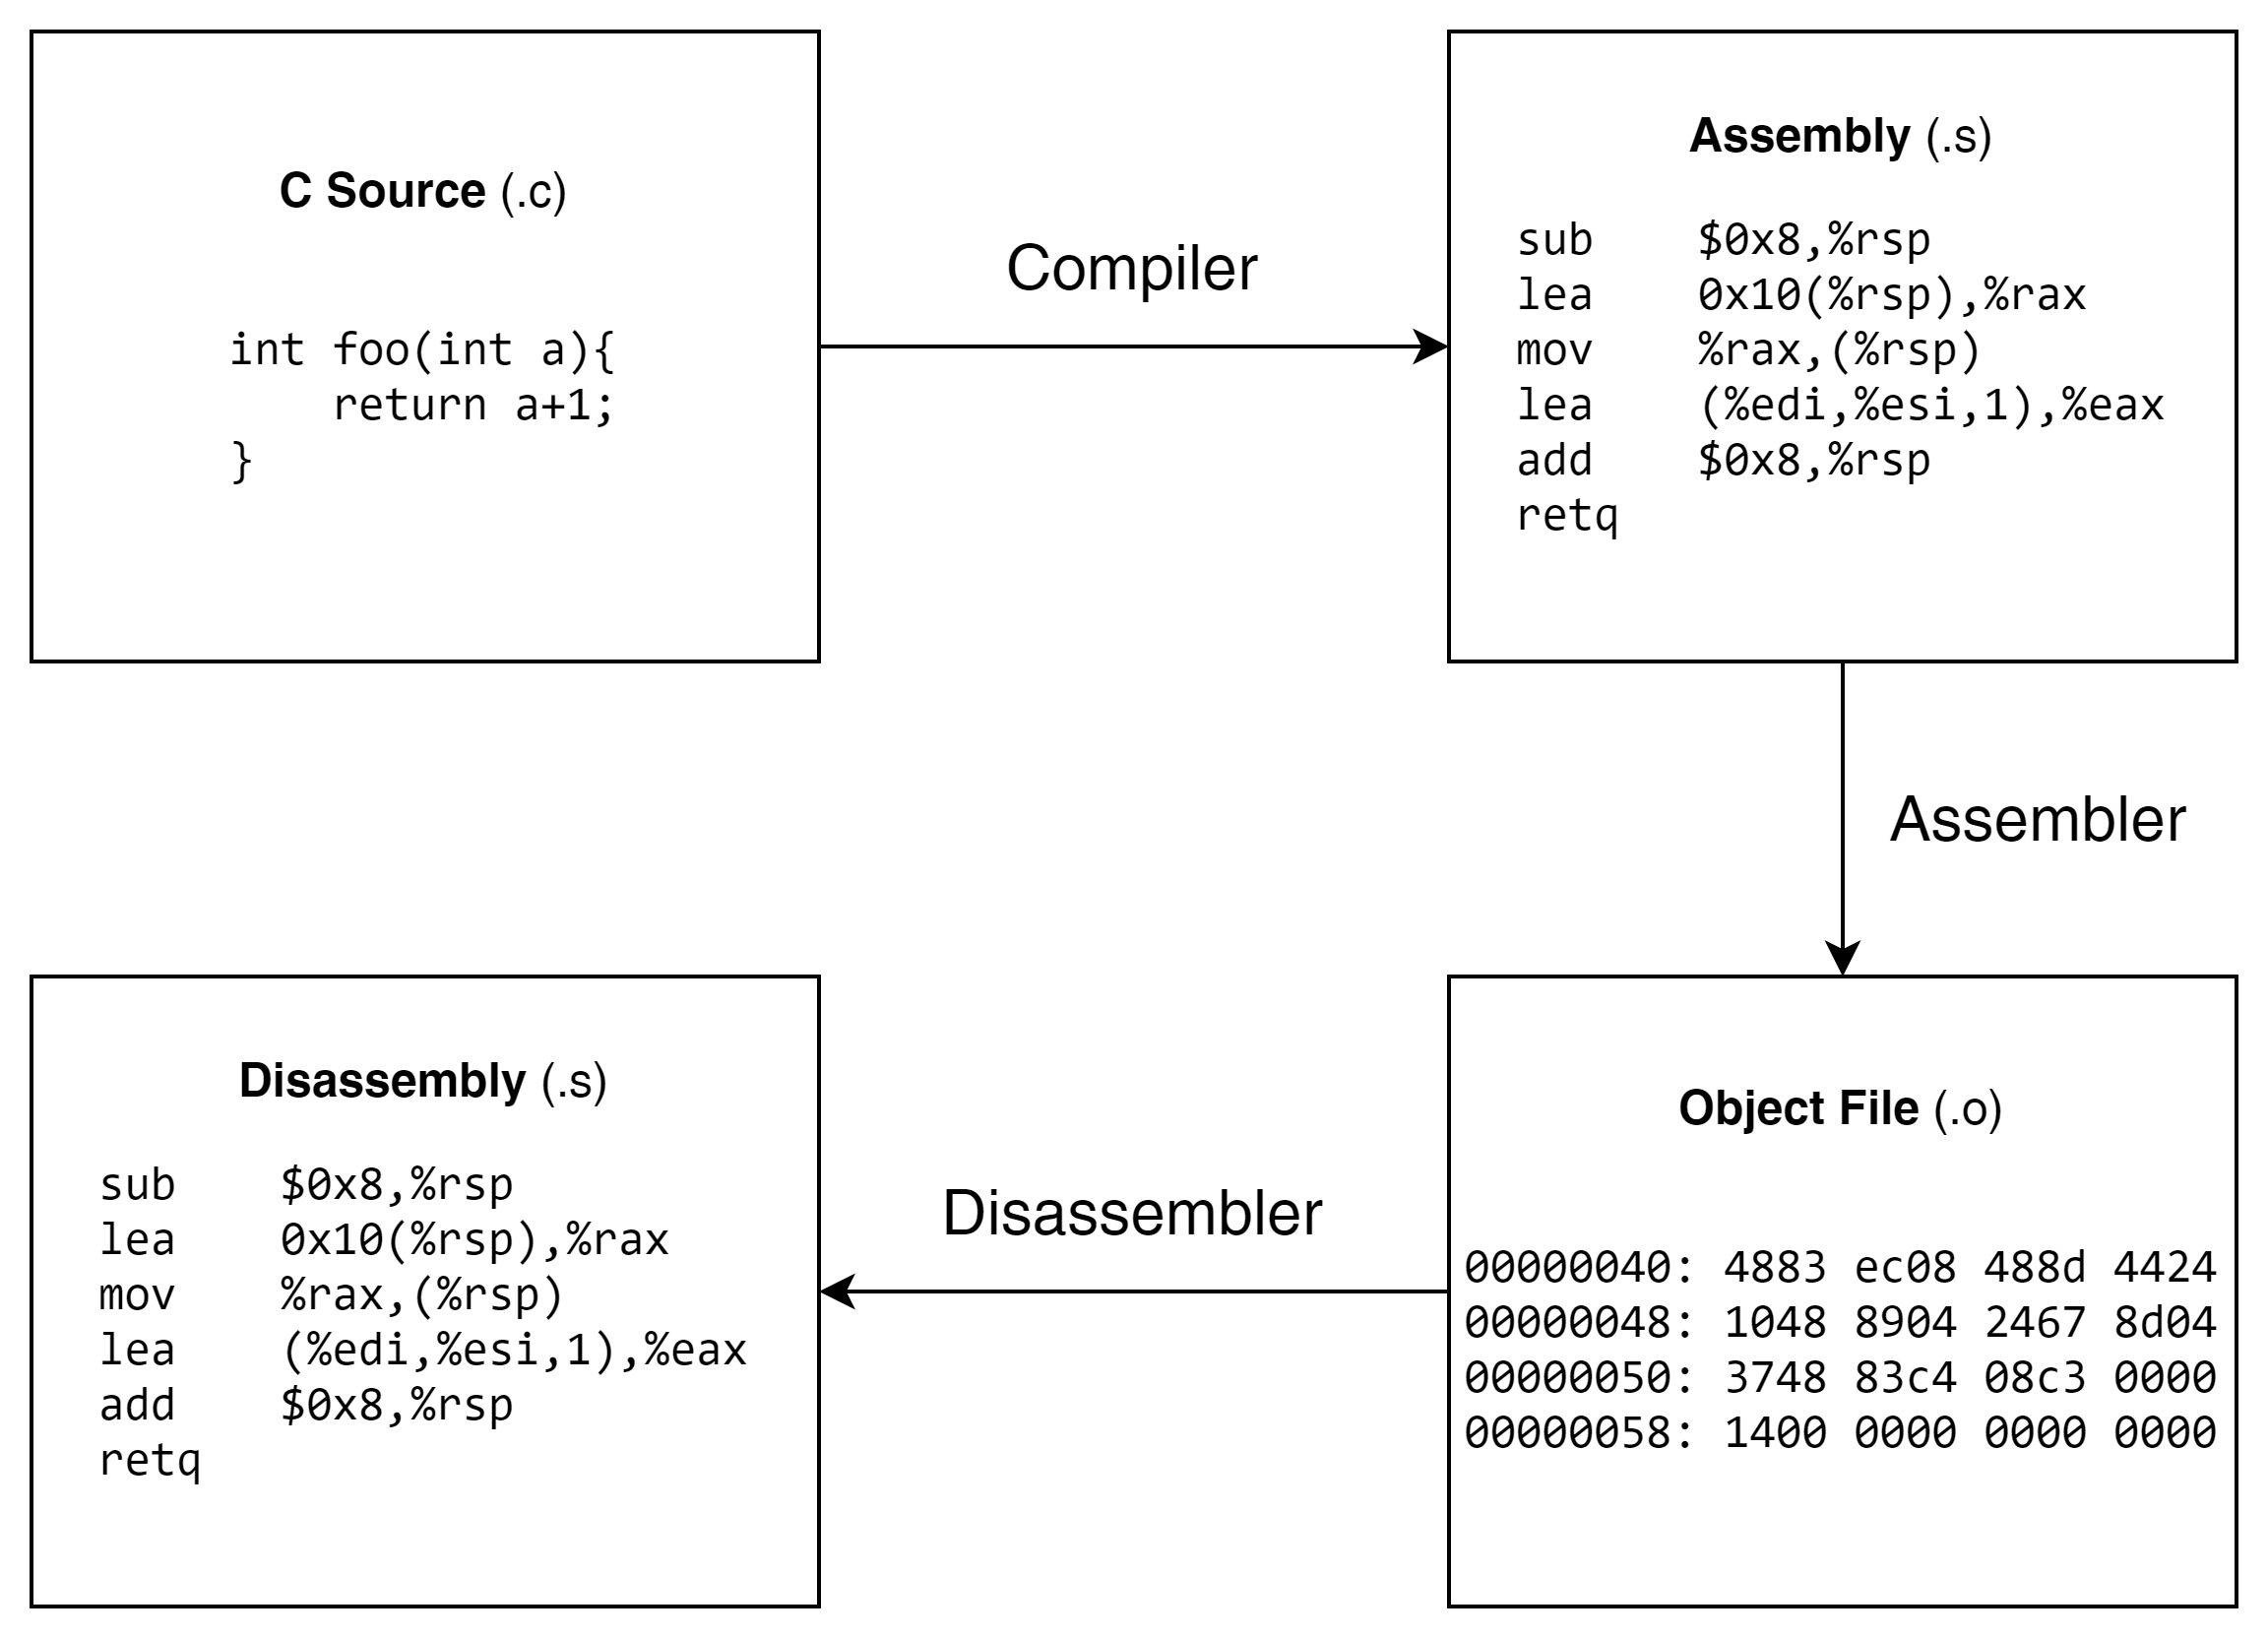
\includegraphics[width=0.75\textwidth]{disas.png}
\end{center}

% The process of disassembling a binary and correctly resolving function definitions is still unsolved and there are many literary works on the various attempts to push the frontier of disassembling accuracy. The industry standard for disassembling is IDA Pro alongside other disassemblers such as Binary Ninja, Radare2 and BAP. Most of these disassemblers implement variations of recursive descent and linear sweeping to reconstruct the control flow of the binary. Modern disassemblers have a 99\% accuracy at identifying function starts in the disassembly of non optimized binaries, but even the best performing disassemblers drop to 82\% identifying functions in aggressively compiler-optimized binaries\cite{andriesse2016depth}. 

\section{Binary Analysis Platform}\label{BAP}
The Carnegie Mellon University Binary Analysis Platform (CMU BAP)\cite{brumley2011bap} is a framework for performing analysis of compiled binary files. The framework comes with various utilities and libraries to analyse binaries, however the framework is mainly designed to be extensible with custom written plugins.

The BAP framework was initially chosen for the disassembly stage for two reasons. Firstly, BAP is written in OCaml and should therefore have a simple integration system with the CompCert project. Secondly, BAP has a system for performing \textit{passes} on assembly after it has been disassembled. This can be used for control flow reconstruction and reconstruction of the starts and relocations of heavily optimized functions. 

As the project developed, extracting the instruction specific mnemonics became an important task, and the BAP default output for instruction names and operands suited the needs of the project perfectly. A workaround to the integration issue was found by running BAP as a separate process and formatting the output of BAP to exactly match the required input to the project.

The BAP framework is designed for automated binary analysis and as such has large performance considerations making the framework an ideal candidate for use in this project. 

% The project is aiming to support object files (\textit{.o} files) for linking. These are similar to a compiled program; they contain compiled instructions, but they do not contain any executable code and haven't had any of the function calls linked. Object files very often (for the purposes of this project, always) contain relocation and linking information which is used to link the function calls inside the object file and linking calls in a compiled binary to the object's function. 


% \section{Expected Hurdles}
% The project has a few notable problems in implementing the project. Firstly CompCert is a massive project, and learning how the compiler is structured and finding where the code injection points should be will require a moderate understanding of how the Assembly and Interpreter are defined in CompCert. CompCert being large will also hinder integration with other OCaml libraries due to having to understand and edit custom makefiles for the project. 

% Calling functions from inside the assembly is another large area for issues to appear, as CompCert requires function calls to have a definition of the target function, and internal function calls inside the assembly will be unlikely to have the required information to correctly re-produce the details of the function call.

